\subsection{Problem}

\renewcommand{\theequation}{\theenumi}
\begin{enumerate}[label=\thesection.\arabic*.,ref=\thesection.\theenumi]
\numberwithin{equation}{enumi}
\item Bag I contains 3 red and 4 black balls while another Bag II contains 5 red and 6 black balls. One ball is drawn at random from one of the bags and it is found to be red. Find the
probability that it was drawn from Bag II.
\\

\solution Let $E_1$ and $E_2$ denote the events of selecting bag-1 and bag-2 respectively. Let A and B denote the events of selecting a red ball and black ball respectively. We need to find the probability of drawing a ball from bag-2 if it is red.i.e.$P\brak{\frac{E_2}{A}}$.
\begin{align}
P\brak{E_1} = \frac{1}{2}\\
P\brak{E_2} = \frac{1}{2}
\end{align}

\begin{align}
P\brak{\frac{A}{E_1}} &= P\brak{\text{Selecting red ball from bag1}}\\
P\brak{\frac{A}{E_1}} &= \frac{3}{7}
\end{align}

\begin{align}
P\brak{\frac{A}{E_2}} &= P\brak{\text{Selecting red ball from bag2}}\\
P\brak{\frac{A}{E_2}} &= \frac{5}{11}
\end{align}

\begin{align}
P\brak{\frac{E_2}{A}} &= \frac{P\brak{E_2}.P\brak{\frac{A}{E_2}}}{P\brak{E_1}.P\brak{\frac{A}{E_1}} + P\brak{E_2}.P\brak{\frac{A}{E_2}}}\\
P\brak{\frac{E_2}{A}} &= \frac{\frac{1}{2}.\frac{5}{11}}{\frac{1}{2}.\frac{3}{7} + \frac{1}{2}.\frac{5}{11}}
\end{align}
which is found to be $\frac{35}{68}$.








\begin{comment}
	\begin{lstlisting}
	./codes/lines/q6.py
	\end{lstlisting}
	\begin{figure}[!ht]
	\centering
	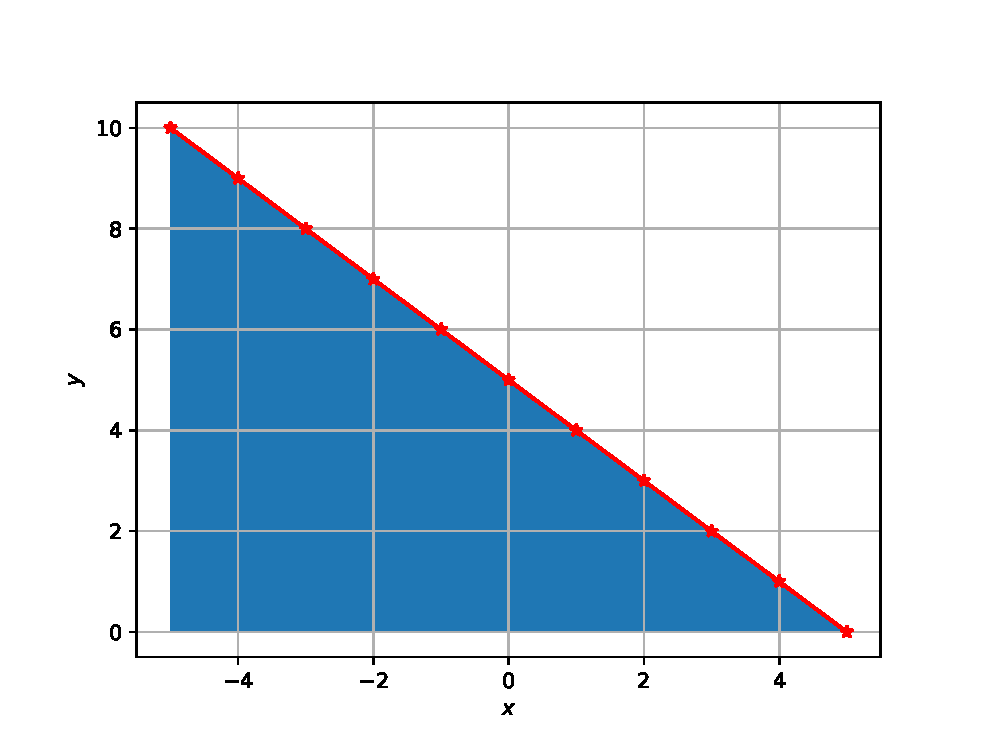
\includegraphics[width=\columnwidth]{./figs/lines/q6.eps}
	\caption{x+y$<$5}
	\label{fig:qsix}	
	\end{figure}
\end{comment}
\end{enumerate}
